\documentclass{report}
\usepackage[utf8]{inputenc}
\usepackage{enumitem}
\title{Assignment 9 (GATE, EC 2017-16)}
\author{Manasa}
\date{December 2020}

\usepackage{circuitikz}


\begin{document}
\maketitle
\section{QUESTION}
\begin{figure}[htp]
        \centering
        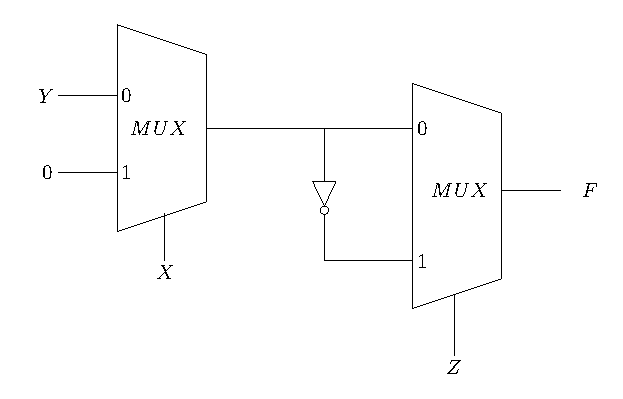
\includegraphics[width=17cm]{Figure.pdf}
         \caption{}
        \label{fig:ok}
\end{figure}
\huge
Consider the circuit shown in the figure.The Boolean expression F implemented by the circuit is

 \begin{enumerate}
 \item X'Y'Z' + XY + Y'Z
\item X'YZ' + XZ + Y'Z
\item X'YZ' + XY + Y'Z
\item X'Y'Z' + XZ + Y'Z
  \end{enumerate}



\section{SOLUTION}
From figure 1,
\newline 
In first multiplexer the input signals are Y and 0,control line is X.According to this the output signal is X'Y
\newline
In second multiplexer the input signals are X'Y and (X'Y)' control line is Z.The output signal is F.
\newline
\newline
F = X'YZ' + ((X'Y)')Z
\newline
\newline
  = X'YZ' + (X + Y')Z   \hspace{3}       (Using demorgan laws)
\newline\newline
= X'YZ' + XZ + Y'Z 
\newline
So the boolean expression F implemented by the circuit is
\newline
\begin{equation}
   \textcolor{blue}{F = X'YZ'+XZ+Y'Z}
\end{equation}
 

\newpage
\section{CIRCUIT}
\begin{figure}[htp]
        \centering
        \includegraphics[width=17cm]{Detailed figure.pdf}
         \caption{}
        \label{fig:ok}
\end{figure}
\newline
From the above figure we can derive the expression of F
\newline
\begin{equation}
   \textcolor{blue}{F = X'YZ'+XZ+Y'Z}
\end{equation}


\newpage
\section{TRUTH TABLE of Expression F}


\begin{table}[]\centering
    \begin{tabular}{|l|l|l|l|}
         \hline
        X & Y & Z & F  \\ \hline
        0 & 0 & 0     & 0  \\
        0 & 0 & 1     & 1  \\
        0 & 1 & 0     & 1   \\ 
        0 & 1 & 1     & 0   \\
        1 & 0 & 0     & 0   \\
        1 & 0 & 1     & 1   \\
        1 & 1 & 0     & 0   \\
        1 & 1 & 1     & 1    \\ 
        \hline

\end{tabular}
\end{table}


\end{document}